%!TEX root = ../../report.tex

\subsection{CityBuilder [NOT DONE]} % (fold)
\label{sub:citybuilder}


CityBuilder is a system introduced by Watson et. al in \cite{Lechner2003} and \cite{Report2004} ``Procedural City Modeling" and ``Procedural Modeling of Land Use in Cities"}. 

It aims to be self automated to minimize necessary input, only needs the terrain description. Although it allows some other input from the user to give some interaction and control. 

To achieve that, it uses agent based simulation to create a system of agents and behaviours that can model specific entities of a city as developers, planning authorities and road builders. The set of rules for each agent is small to achieve a simple behaviour. With that, they what to make their ``model extendible not only in regard to the types of structures that are produced but also in describing the social and cultural influences prevalent in all cities."

\begin{figure}[htbp]
	\centering
	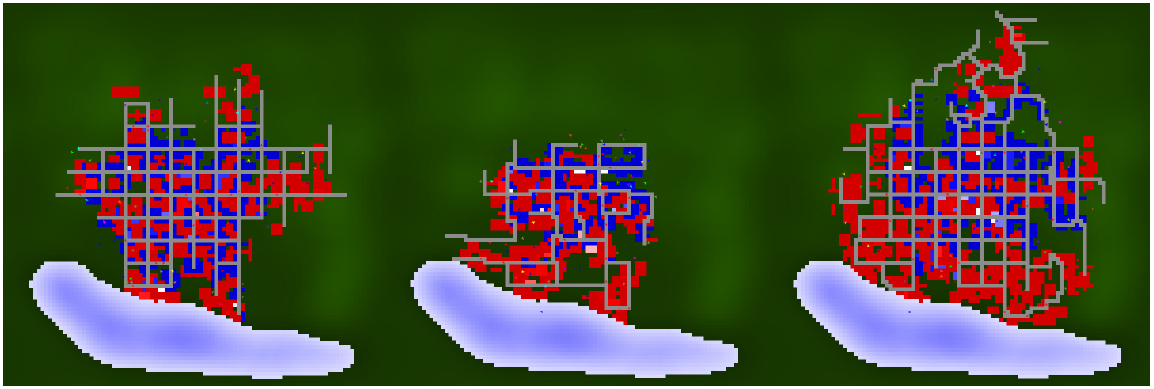
\includegraphics[width=0.95\textwidth]{img/AgentBased-ProceduralCityMod/DifferentCityLayouts.PNG}
	\caption{Different Road Netowrks}
	\label{fig:label}
\end{figure}

\subsubsection{Road Network} % (fold)
\label{ssub:road_network}
The road network is designed by the agents based on the input terrain description wish will describe the height map and forbidden areas for roads, as water. 

The user can specify that the roads must follow a pre-established gridded pattern, or give the freedom to network to grow more organic. The image presents this two options and a combination of the two with a centre with a gridded pattern ant organic surroundings.


There are two types of road building agents, the \emph{extenders} and the \emph{connectors}:

\begin{itemize}
	\item[extenders] The \emph{extenders} search the area around exiting developments to look for areas that are not being served by any road to expand the current road network.
	
	\item[connectors] The \emph{connectors} roam trough existing roads and sampling random points in the road network within a given radius. It tries to reach that point trough the road via a BSF. If it cannot reach or the distance needed is over a threshold value, the agent tries to create a road between these two points.
\end{itemize}




% subsubsection road_network (end)

\subsubsection{Buildings} % (fold)
\label{ssub:buildings}

This system does not develop buildings, but it's developer agents generate parcels and specify the use of the land. They can identify ``at least nine different types of land usages". They perform the role of urban developers that buy land, request planing permission, build and sell. They track the usage of their lands and specify the parameters to the buildings that can be build there.

% subsubsection buildings (end)

\subsubsection{The City} % (fold)
\label{ssub:the_city}

This system develop an evolving conceptual model of one city, that can represent the growth and evolution of a city through the time. 

% subsubsection the_city (end)

% subsection citybuilder (end)
